\documentclass[aspectratio=169,11pt]{beamer}
% =====================================================================
% Proyecto Integrador ML1 · Segunda entrega (Fase 2)
% Pronóstico de la demanda minorista de muebles en Colombia
% Compilar con pdfLaTeX. Los datos de las gráficas están en datos/.
% =====================================================================
\usepackage[T1]{fontenc}
\usepackage[utf8]{inputenc}
\usepackage{lmodern}
\usepackage{booktabs}
\usepackage{amssymb}
\usepackage{array}
\usepackage{tikz}
\usetikzlibrary{arrows.meta,positioning,calc,fit,backgrounds,shapes.geometric,decorations.pathreplacing}
\usepackage{pgfplots}
\pgfplotsset{compat=1.18}

% ---------------- Integrantes: cámbienlos solo aquí ----------------
\newcommand{\integrantes}{Santiago Bernal Rozo \quad·\quad Joshua Samad Trujillo Lagos}
\newcommand{\integrantesCorto}{Bernal y Trujillo}
\newcommand{\repositorio}{github.com/JojjjT/Machine-Learning-1}

% ---------------- Colores ----------------
\definecolor{navy}{HTML}{14213D}
\definecolor{azul}{HTML}{1F5FAF}
\definecolor{azulc}{HTML}{EAF1FA}
\definecolor{naranja}{HTML}{C0571F}
\definecolor{naranjac}{HTML}{FBEFE9}
\definecolor{verde}{HTML}{2E7D4F}
\definecolor{verdec}{HTML}{E8F3EC}
\definecolor{gris}{HTML}{5F6673}
\definecolor{grisc}{HTML}{ECEAE3}
\definecolor{linea}{HTML}{D6D2C7}
\definecolor{fondo}{HTML}{F7F6F2}
\definecolor{tarjeta}{HTML}{FDFCFA}

% ---------------- Estilo ----------------
\setbeamertemplate{navigation symbols}{}
\setbeamercolor{background canvas}{bg=fondo}
\setbeamercolor{normal text}{fg=navy}
\setbeamercolor{structure}{fg=azul}
\setbeamercolor{itemize item}{fg=naranja}
\setbeamercolor{itemize subitem}{fg=naranja}
\setbeamertemplate{itemize item}{\small\raise0.15ex\hbox{\textbullet}}
\setbeamertemplate{itemize subitem}{\scriptsize\raise0.2ex\hbox{--}}
\setlength{\leftmargini}{1.1em}
\makeatletter
\setbeamertemplate{frametitle}{%
  \vspace*{0.35cm}%
  \ifx\insertframesubtitle\@empty\else
    {\color{naranja}\fontsize{7}{8}\selectfont\bfseries\MakeUppercase{\insertframesubtitle}}\par\vspace{0.12cm}%
  \fi
  {\color{navy}\fontsize{15}{17}\selectfont\bfseries\insertframetitle}\par}
\makeatother
\setbeamertemplate{footline}{%
  \leavevmode\hbox to \paperwidth{\hspace{0.55cm}{\color{gris}\fontsize{6}{7}\selectfont Proyecto Integrador · Machine Learning I · \integrantesCorto}\hfill
  {\color{gris}\fontsize{6}{7}\selectfont\insertframenumber\,/\,\inserttotalframenumber}\hspace{0.55cm}}\vspace{0.28cm}}

\pgfkeys{/pgf/number format/.cd,use comma,1000 sep={.}}
\pgfplotsset{
  base/.style={axis line style={gris!70}, tick style={gris!70}, tick label style={font=\tiny,color=gris},
    label style={font=\scriptsize,color=navy}, title style={font=\scriptsize\bfseries,color=navy},
    legend style={font=\tiny,draw=none,fill=none}, grid style={linea!70}},
}
\tikzset{
  caja/.style={draw=linea, fill=tarjeta, rounded corners=3pt, align=center, font=\scriptsize, inner sep=4pt},
  cajaaz/.style={draw=azul, fill=azulc, rounded corners=3pt, align=center, font=\scriptsize, inner sep=4pt},
  cajana/.style={draw=naranja, fill=naranjac, rounded corners=3pt, align=center, font=\scriptsize, inner sep=4pt},
  cajave/.style={draw=verde, fill=verdec, rounded corners=3pt, align=center, font=\scriptsize, inner sep=4pt},
  cajanavy/.style={fill=navy, text=white, rounded corners=3pt, align=center, font=\scriptsize\bfseries, inner sep=4pt},
  flecha/.style={-{Stealth[length=5pt]}, thick, gris},
}
\newcommand{\dato}[2]{{\color{azul}\bfseries #1}\,{\scriptsize #2}}
\newcommand{\nota}[1]{{\color{gris}\scriptsize #1}}

\hyphenpenalty=10000
\exhyphenpenalty=10000

\begin{document}

% =====================================================================
% 1. Portada
% =====================================================================
\begin{frame}[plain]
\begin{tikzpicture}[remember picture,overlay]
  \fill[navy] (current page.south west) rectangle (current page.north east);
  % motivo: serie con estacionalidad y la caída de 2020
  \begin{scope}[shift={($(current page.south east)+(-5.75,2.2)$)}, x=0.088cm, y=0.04cm]
    \draw[azul!80, line width=1pt] plot[smooth, tension=0.4] file {datos/serie_portada.txt};
  \end{scope}
  \node[anchor=north west, text width=12.4cm, align=left] at ($(current page.north west)+(0.9,-0.85)$) {%
    {\color{azul!45}\fontsize{7.5}{9}\selectfont\bfseries PROYECTO INTEGRADOR · SEGUNDA ENTREGA}\\[0.35cm]
    {\color{white}\fontsize{22}{25}\selectfont\bfseries Pronóstico de la demanda minorista\\[0.05cm] de muebles en Colombia}\\[0.35cm]
    {\color{white!80!azul}\fontsize{10}{12}\selectfont Fase 2: datos, modelamiento y validación}\\[0.15cm]
    {\color{white!70!azul}\fontsize{8}{10}\selectfont Reproducción de İnce y Taşdemir (2024) con modelos de Machine Learning I}};
  \node[anchor=south west, text width=12cm, align=left] at ($(current page.south west)+(0.9,0.75)$) {%
    {\color{white}\fontsize{9}{11}\selectfont\bfseries \integrantes}\\[0.12cm]
    {\color{white!65!azul}\fontsize{7}{9}\selectfont Machine Learning I · Prof. Alber Montenegro · Universidad Externado de Colombia · 2026}\\[0.05cm]
    {\color{white!65!azul}\fontsize{7}{9}\selectfont Código: \repositorio}};
\end{tikzpicture}
\end{frame}

% =====================================================================
% 2. Correcciones
% =====================================================================
\begin{frame}{Qué corregimos frente a la primera entrega}{Punto de partida}
\vspace{0.15cm}
\begin{center}
\begin{tikzpicture}[x=1cm,y=1cm]
  \node[font=\scriptsize\bfseries,color=gris] at (2.1,0.55) {Antes};
  \node[font=\scriptsize\bfseries,color=navy] at (9.3,0.55) {Ahora};
  \foreach \i/\tema/\antes/\ahora in {
    0/{Tamaño}/{60 observaciones mensuales}/{Panel mes × ciudad × subsector: \textbf{5.400 filas}},
    1/{Modelos}/{Holt–Winters y otros fuera del curso}/{Solo regresión lineal múltiple, Ridge y KNN},
    2/{Código}/{No había código ejecutable}/{Scripts reproducibles con semilla 42},
    3/{Línea base}/{Solo descrita}/{Construida y corrida: \textbf{MAPE 11,03\,\%}},
    4/{Métrica}/{MAPE «porque es lo usual»}/{MAPE justificado por el costo del inventario}} {
    \node[caja, text width=3.6cm, minimum height=0.62cm, text=gris] (a\i) at (2.1,-\i*0.82) {\antes};
    \node[cajaaz, text width=6.4cm, minimum height=0.62cm, text=navy] (b\i) at (9.3,-\i*0.82) {\ahora};
    \draw[flecha] (a\i.east) -- (b\i.west);
    \node[font=\tiny\bfseries, color=naranja, anchor=east] at (-0.05,-\i*0.82) {\tema};
  }
\end{tikzpicture}
\end{center}
\vspace{0.1cm}
\centering\nota{Los cinco puntos salen de la retroalimentación de la primera entrega.}
\end{frame}

% =====================================================================
% 3. El artículo base
% =====================================================================
\begin{frame}{El artículo: regresión lineal frente a Holt–Winters}{El artículo base}
\begin{columns}[T,onlytextwidth]
\column{0.42\textwidth}
\small
{\color{gris}\scriptsize İnce y Taşdemir (2024), \emph{Systems}, 12(6), 219}
\begin{itemize}\setlength{\itemsep}{3pt}
  \item Ventas minoristas mensuales de muebles en EE.\,UU.
  \item 60 meses, de 2019 a 2023, con la pandemia adentro.
  \item Nueve variables candidatas; la selección \emph{stepwise} deja las útiles.
  \item Pronóstico a 36 meses (2024–2026).
\end{itemize}
\vspace{0.15cm}
{\color{azul}\bfseries Conclusión:} la regresión lineal múltiple predice mejor (R$^2$ = 76,73\,\%).
\column{0.55\textwidth}
\vspace{0.1cm}
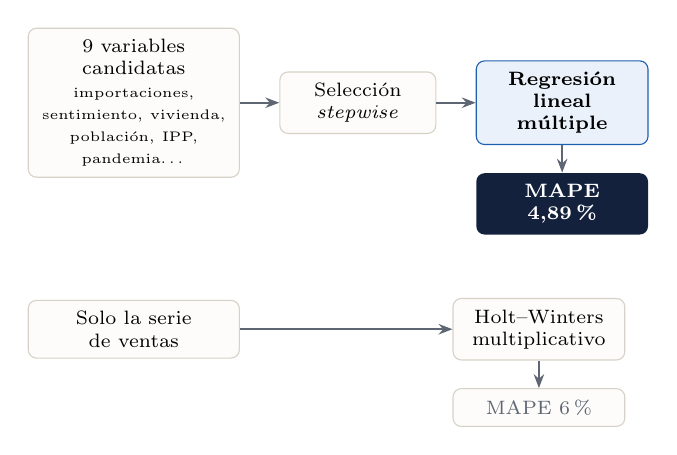
\begin{tikzpicture}[node distance=0.45cm and 0.5cm]
  \node[caja, text width=2.4cm] (vars) {9 variables candidatas\\ \tiny importaciones, sentimiento, vivienda, población, IPP, pandemia\dots};
  \node[caja, right=of vars, text width=1.7cm] (step) {Selección\\ \emph{stepwise}};
  \node[cajaaz, right=of step, text width=1.9cm] (mlr) {\bfseries Regresión lineal múltiple};
  \node[cajanavy, below=0.35cm of mlr, text width=1.9cm] (m1) {MAPE 4,89\,\%};
  \node[caja, below=1.55cm of vars, text width=2.4cm] (serie) {Solo la serie de ventas};
  \node[caja, right=of serie, xshift=2.2cm, text width=1.9cm] (hw) {Holt–Winters multiplicativo};
  \node[caja, below=0.35cm of hw, text width=1.9cm, text=gris] (m2) {MAPE 6\,\%};
  \draw[flecha] (vars) -- (step); \draw[flecha] (step) -- (mlr); \draw[flecha] (mlr) -- (m1);
  \draw[flecha] (serie) -- (hw); \draw[flecha] (hw) -- (m2);
\end{tikzpicture}
\end{columns}
\end{frame}

% =====================================================================
% 4. Problema supervisado y panel
% =====================================================================
\begin{frame}{Nuestro problema: un panel de 5.400 filas}{Planteamiento en Colombia}
\begin{columns}[T,onlytextwidth]
\column{0.47\textwidth}
\small
\begin{itemize}\setlength{\itemsep}{4pt}
  \item {\bfseries Tarea:} regresión.
  \item {\bfseries Objetivo:} ventas mensuales de muebles, en millones de USD.
  \item {\bfseries Unidad:} un mes, en una ciudad, en un subsector.
  \item {\bfseries 9 predictoras:} importaciones, sentimiento del consumidor, inicios de vivienda, población, IPP, pandemia, ciudad, subsector y mes.
\end{itemize}
\vspace{0.1cm}
\colorbox{naranjac}{\parbox{0.95\linewidth}{\scriptsize\textbf{¿Por qué un panel?} La guía pide 5.000 registros. Una serie nacional mensual necesitaría más de 400 años de historia.}}
\column{0.5\textwidth}
\centering
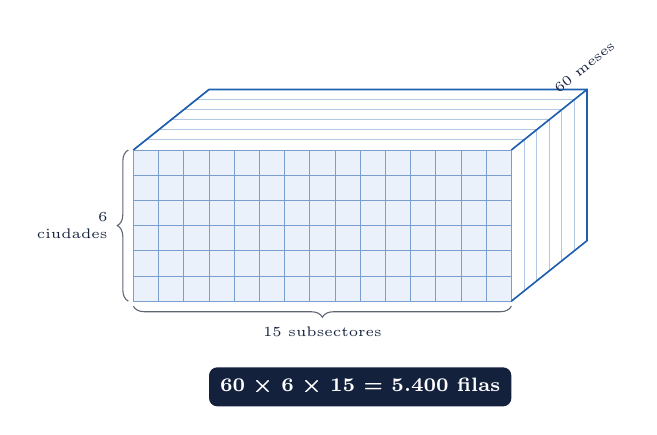
\begin{tikzpicture}[x=0.32cm,y=0.32cm]
  % cara frontal: ciudades (filas) × subsectores (columnas)
  \foreach \c in {0,...,14} \foreach \r in {0,...,5}
    \fill[azulc, draw=azul!60, line width=0.3pt] (\c,\r) rectangle ++(1,1);
  % profundidad: meses
  \foreach \k in {1,...,6} {
    \draw[azul!35, line width=0.3pt] (15+\k*0.5,6+\k*0.4) -- (\k*0.5,6+\k*0.4);
    \draw[azul!35, line width=0.3pt] (15+\k*0.5,6+\k*0.4) -- (15+\k*0.5,\k*0.4);
  }
  \draw[azul, line width=0.6pt] (0,6) -- (3,8.4) -- (18,8.4) -- (18,2.4) -- (15,0);
  \draw[azul, line width=0.6pt] (15,6) -- (18,8.4);
  \draw[decorate,decoration={brace,amplitude=4pt,mirror},gris] (0,-0.2) -- (15,-0.2) node[midway,below=4pt,font=\tiny,text=navy] {15 subsectores};
  \draw[decorate,decoration={brace,amplitude=4pt},gris] (-0.2,0) -- (-0.2,6) node[midway,left=4pt,font=\tiny,text=navy,align=right] {6\\ciudades};
  \node[font=\tiny, text=navy, rotate=38.7] at (17.9,9.3) {60 meses};
  \node[cajanavy, font=\scriptsize\bfseries] at (9,-3.4) {60 × 6 × 15 = 5.400 filas};
\end{tikzpicture}
\end{columns}
\end{frame}

% =====================================================================
% 5. Cómo se simularon los datos
% =====================================================================
\begin{frame}{Cómo simulamos los datos}{Simulación fundamentada}
\vspace{0.05cm}
\centering
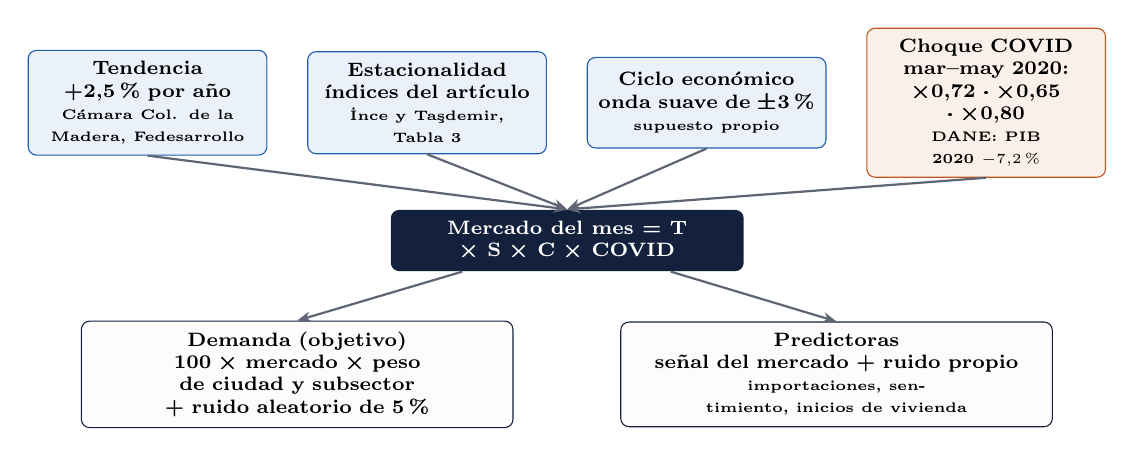
\begin{tikzpicture}[x=1cm,y=1cm]
  \node[cajaaz, text width=2.75cm, minimum height=1.15cm] (t) at (0,0) {\bfseries Tendencia\\ +2,5\,\% por año\\ \tiny Cámara Col. de la Madera, Fedesarrollo};
  \node[cajaaz, text width=2.75cm, minimum height=1.15cm] (s) at (3.55,0) {\bfseries Estacionalidad\\ índices del artículo\\ \tiny İnce y Taşdemir, Tabla 3};
  \node[cajaaz, text width=2.75cm, minimum height=1.15cm] (c) at (7.1,0) {\bfseries Ciclo económico\\ onda suave de ±3\,\%\\ \tiny supuesto propio};
  \node[cajana, text width=2.75cm, minimum height=1.15cm] (v) at (10.65,0) {\bfseries Choque COVID\\ mar–may 2020:\\ ×0,72 · ×0,65 · ×0,80\\ \tiny DANE: PIB 2020 $-7{,}2\,\%$};
  \node[cajanavy, text width=4.2cm, minimum height=0.7cm] (m) at (5.33,-1.75) {Mercado del mes = T × S × C × COVID};
  \foreach \n in {t,s,c,v} \draw[flecha] (\n.south) -- (m.north);
  \node[caja, text width=5.2cm, minimum height=1.1cm, draw=navy] (d) at (1.9,-3.45) {\bfseries Demanda (objetivo)\\ 100 × mercado × peso de ciudad y subsector\\ + ruido aleatorio de 5\,\%};
  \node[caja, text width=5.2cm, minimum height=1.1cm, draw=navy] (p) at (8.75,-3.45) {\bfseries Predictoras\\ señal del mercado + ruido propio\\ \tiny importaciones, sentimiento, inicios de vivienda};
  \draw[flecha] (m) -- (d.north); \draw[flecha] (m) -- (p.north);
\end{tikzpicture}

\vspace{0.12cm}
\nota{El ruido es la parte que ningún modelo puede adivinar: por eso el R$^2$ no llega a 1, como en datos reales.}
\end{frame}

% =====================================================================
% 6. Verificación 1: estructura temporal
% =====================================================================
\begin{frame}{La simulación reproduce la estructura temporal}{Verificación de la simulación (1)}
\begin{columns}[T,onlytextwidth]
\column{0.55\textwidth}
\begin{tikzpicture}
\begin{axis}[base, width=8.4cm, height=5.0cm, xmin=1, xmax=60, ymin=60, ymax=125,
  xtick={1,13,25,37,49}, xticklabels={2019,2020,2021,2022,2023}, ylabel={Ventas promedio (millones USD)},
  title={Ventas promedio por mes, 2019–2023}, grid=major]
  \fill[naranja!15] (axis cs:14.5,60) rectangle (axis cs:17.5,125);
  \addplot[azul, line width=1pt, mark=none] table[x=t,y=y,col sep=comma] {datos/serie.csv};
  \node[font=\tiny, text=naranja, anchor=west, align=left] at (axis cs:18,72) {abril de 2020:\\ $-31\,\%$ frente a 2019};
\end{axis}
\end{tikzpicture}
\column{0.43\textwidth}
\begin{tikzpicture}
\begin{axis}[base, width=6.4cm, height=5.0cm, xmin=0.5, xmax=12.5, ymin=0.88, ymax=1.08,
  xtick={1,...,12}, xticklabels={E,F,M,A,M,J,J,A,S,O,N,D}, title={Índice estacional},
  yticklabel style={/pgf/number format/fixed,/pgf/number format/precision=2}, grid=major,
  legend pos=south east]
  \addplot[gris, dashed, line width=0.9pt, mark=*, mark size=1pt] table[x=mes,y=paper,col sep=comma] {datos/estacional.csv};
  \addplot[azul, line width=1pt, mark=*, mark size=1.2pt] table[x=mes,y=sim,col sep=comma] {datos/estacional.csv};
  \legend{Artículo, Simulación}
\end{axis}
\end{tikzpicture}
\end{columns}
\vspace{0.05cm}
\centering\nota{El índice recuperado de los datos difiere como máximo 0,019 del publicado en el artículo.}
\end{frame}

% =====================================================================
% 7. Verificación 2: relaciones y calidad
% =====================================================================
\begin{frame}{Las correlaciones se parecen a las del artículo}{Verificación de la simulación (2)}
\begin{columns}[T,onlytextwidth]
\column{0.58\textwidth}
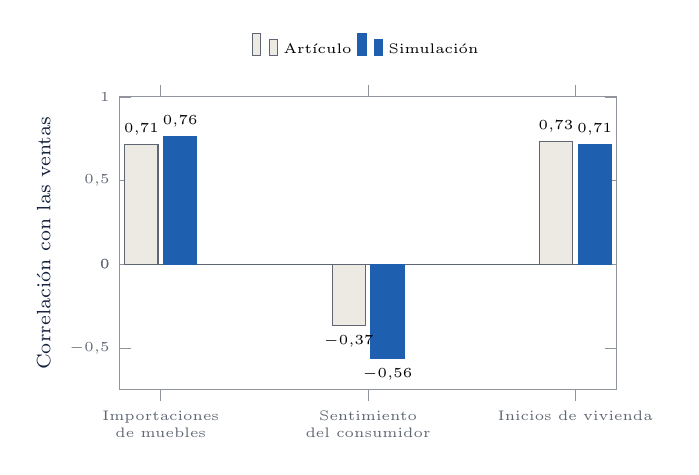
\begin{tikzpicture}
\begin{axis}[base, ybar, width=7.9cm, height=5.3cm, bar width=12pt, ymin=-0.75, ymax=1,
  symbolic x coords={Importaciones,Sentimiento,Vivienda}, xtick=data,
  xticklabels={Importaciones de muebles, Sentimiento del consumidor, Inicios de vivienda},
  x tick label style={font=\tiny, text width=2.2cm, align=center},
  ylabel={Correlación con las ventas},
  nodes near coords, nodes near coords style={font=\tiny, /pgf/number format/fixed, /pgf/number format/precision=2},
  legend style={at={(0.5,1.02)}, anchor=south, legend columns=2, yshift=8pt}, extra y ticks={0}, extra y tick style={grid=major, grid style={gris}}]
  \addplot[fill=grisc, draw=gris] coordinates {(Importaciones,0.714) (Sentimiento,-0.366) (Vivienda,0.731)};
  \addplot[fill=azul, draw=azul] coordinates {(Importaciones,0.763) (Sentimiento,-0.564) (Vivienda,0.714)};
  \legend{Artículo, Simulación}
\end{axis}
\end{tikzpicture}
\column{0.39\textwidth}
\vspace{0.2cm}
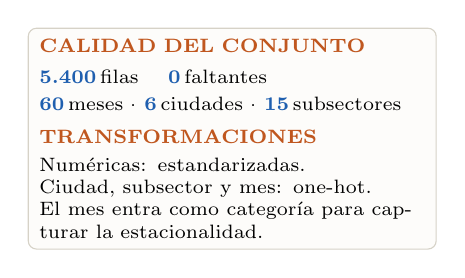
\begin{tikzpicture}
  \node[caja, text width=4.9cm, align=left, font=\scriptsize] {%
    {\color{naranja}\bfseries CALIDAD DEL CONJUNTO}\\[3pt]
    \dato{5.400}{filas} \quad \dato{0}{faltantes}\\[2pt]
    \dato{60}{meses} · \dato{6}{ciudades} · \dato{15}{subsectores}\\[4pt]
    {\color{naranja}\bfseries TRANSFORMACIONES}\\[2pt]
    Numéricas: estandarizadas.\\ Ciudad, subsector y mes: one-hot.\\ El mes entra como categoría para capturar la estacionalidad.};
\end{tikzpicture}
\vspace{0.2cm}

\scriptsize Mismos signos y magnitudes parecidas. El sentimiento quedó más fuerte que en el artículo ($-0{,}56$ frente a $-0{,}37$).
\end{columns}
\end{frame}

% =====================================================================
% 8. Flujo sin fuga
% =====================================================================
\begin{frame}{Un flujo sin fuga de información}{Flujo reproducible}
\centering
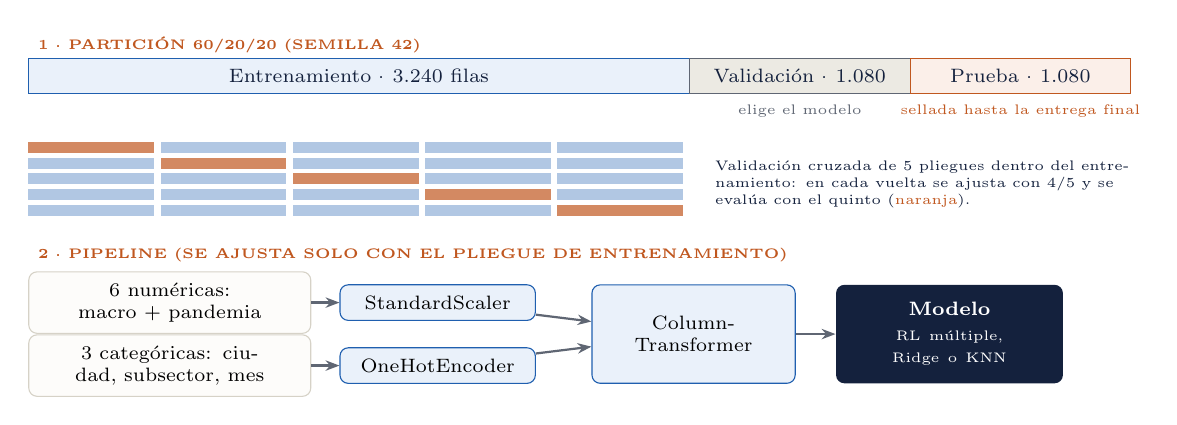
\begin{tikzpicture}[x=1cm,y=1cm]
  % partición
  \node[font=\tiny\bfseries, color=naranja, anchor=west] at (0,0.62) {1 · PARTICIÓN 60/20/20 (SEMILLA 42)};
  \draw[fill=azulc, draw=azul] (0,0) rectangle (8.4,0.45) node[midway, font=\scriptsize, text=navy] {Entrenamiento · 3.240 filas};
  \draw[fill=grisc, draw=gris] (8.4,0) rectangle (11.2,0.45) node[midway, font=\scriptsize, text=navy] {Validación · 1.080};
  \draw[fill=naranjac, draw=naranja] (11.2,0) rectangle (14,0.45) node[midway, font=\scriptsize, text=navy] {Prueba · 1.080};
  \node[font=\tiny, text=naranja, anchor=north] at (12.6,-0.02) {sellada hasta la entrega final};
  \node[font=\tiny, text=gris, anchor=north] at (9.8,-0.02) {elige el modelo};
  % validación cruzada
  \foreach \k in {0,...,4} {
    \foreach \j in {0,...,4} {
      \pgfmathsetmacro{\col}{ifthenelse(\k==\j,1,0)}
      \ifdim\col pt=1pt \fill[naranja!70] (\j*1.68,-0.75-\k*0.2) rectangle ++(1.6,0.14);
      \else \fill[azul!35] (\j*1.68,-0.75-\k*0.2) rectangle ++(1.6,0.14); \fi
    }
  }
  \node[font=\tiny, text=navy, anchor=west, align=left, text width=5.3cm] at (8.6,-1.15) {Validación cruzada de 5 pliegues dentro del entrenamiento: en cada vuelta se ajusta con 4/5 y se evalúa con el quinto ({\color{naranja}naranja}).};
  % pipeline
  \node[font=\tiny\bfseries, color=naranja, anchor=west] at (0,-2.05) {2 · PIPELINE (SE AJUSTA SOLO CON EL PLIEGUE DE ENTRENAMIENTO)};
  \node[caja, text width=3.3cm, anchor=west] (num) at (0,-2.65) {6 numéricas: macro + pandemia};
  \node[caja, text width=3.3cm, anchor=west] (cat) at (0,-3.45) {3 categóricas: ciudad, subsector, mes};
  \node[cajaaz, text width=2.2cm] (sc) at (5.2,-2.65) {StandardScaler};
  \node[cajaaz, text width=2.2cm] (oh) at (5.2,-3.45) {OneHotEncoder};
  \node[cajaaz, text width=2.3cm, minimum height=1.25cm] (ct) at (8.45,-3.05) {Column-\\Transformer};
  \node[cajanavy, text width=2.6cm, minimum height=1.25cm] (mo) at (11.7,-3.05) {Modelo\\[1pt] \tiny\mdseries RL múltiple, Ridge o KNN};
  \draw[flecha] (num) -- (sc); \draw[flecha] (cat) -- (oh);
  \draw[flecha] (sc) -- (ct); \draw[flecha] (oh) -- (ct); \draw[flecha] (ct) -- (mo);
\end{tikzpicture}

\vspace{0.12cm}
\nota{Ninguna media, desviación o categoría se calcula con datos de validación o de prueba.}
\end{frame}

% =====================================================================
% 9. Líneas base
% =====================================================================
\begin{frame}{Primero, el piso: dos líneas base corridas}{Línea base}
\begin{columns}[c,onlytextwidth]
\column{0.53\textwidth}
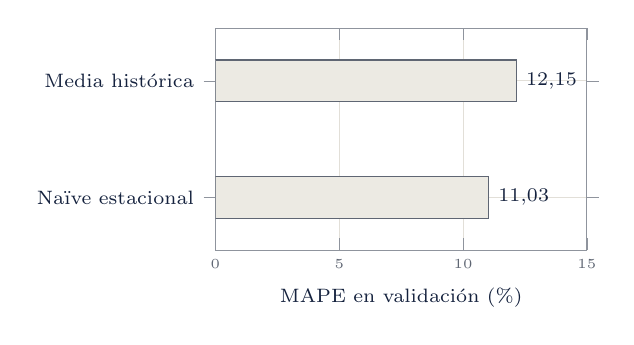
\begin{tikzpicture}
\begin{axis}[base, xbar, width=6.3cm, height=4.4cm, bar width=15pt, xmin=0, xmax=15,
  symbolic y coords={Estacional,Media}, ytick={Estacional,Media}, yticklabels={{Naïve estacional}, {Media histórica}},
  y tick label style={font=\scriptsize, color=navy}, xlabel={MAPE en validación (\%)}, enlarge y limits=0.45,
  nodes near coords, nodes near coords style={font=\scriptsize\bfseries, color=navy, /pgf/number format/fixed, /pgf/number format/precision=2},
  nodes near coords align={horizontal}, grid=major]
  \addplot[fill=grisc, draw=gris] coordinates {(11.03,Estacional) (12.15,Media)};
\end{axis}
\end{tikzpicture}
\column{0.44\textwidth}
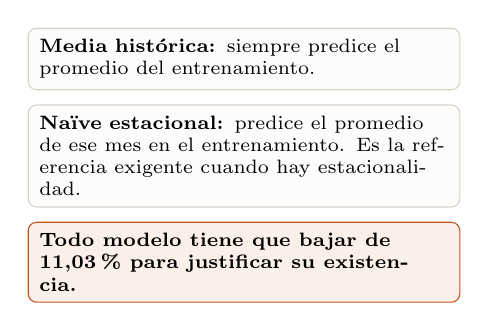
\begin{tikzpicture}
  \node[caja, text width=5.2cm, align=left] (a) {{\bfseries Media histórica:} siempre predice el promedio del entrenamiento.};
  \node[caja, text width=5.2cm, align=left, below=0.18cm of a] (b) {{\bfseries Naïve estacional:} predice el promedio de ese mes en el entrenamiento. Es la referencia exigente cuando hay estacionalidad.};
  \node[cajana, text width=5.2cm, align=left, below=0.18cm of b, font=\scriptsize\bfseries] {Todo modelo tiene que bajar de 11,03\,\% para justificar su existencia.};
\end{tikzpicture}
\end{columns}
\end{frame}

% =====================================================================
% 10. Modelos y ajuste de hiperparámetros
% =====================================================================
\begin{frame}{Tres modelos del curso y su ajuste por validación cruzada}{Entrenamiento}
\begin{columns}[T,onlytextwidth]
\column{0.31\textwidth}
\begin{tikzpicture}
  \node[cajaaz, text width=4.1cm, align=left] (m1) {{\bfseries Regresión lineal múltiple}\\ Una recta con muchas variables. No tiene hiperparámetros.};
  \node[cajaaz, text width=4.1cm, align=left, below=0.16cm of m1] (m2) {{\bfseries Ridge}\\ La misma recta, con coeficientes «frenados» por $\alpha$.};
  \node[cajaaz, text width=4.1cm, align=left, below=0.16cm of m2] (m3) {{\bfseries KNN de regresión}\\ Promedia las ventas de los $k$ casos más parecidos.};
\end{tikzpicture}
\column{0.33\textwidth}
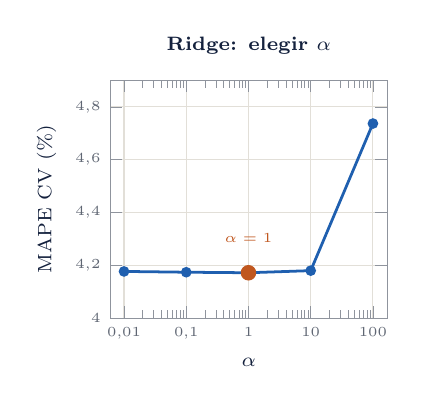
\begin{tikzpicture}
\begin{axis}[base, width=5.1cm, height=4.6cm, xmode=log, xmin=0.006, xmax=170, ymin=4, ymax=4.9,
  xtick={0.01,0.1,1,10,100}, xticklabels={{0,01},{0,1},{1},{10},{100}},
  xlabel={$\alpha$}, ylabel={MAPE CV (\%)}, title={Ridge: elegir $\alpha$}, grid=major,
  yticklabel style={/pgf/number format/fixed,/pgf/number format/precision=1}]
  \addplot[azul, line width=1pt, mark=*, mark size=1.4pt] coordinates {(0.01,4.177) (0.1,4.174) (1,4.172) (10,4.18) (100,4.737)};
  \addplot[only marks, mark=*, mark size=2.6pt, naranja] coordinates {(1,4.172)};
  \node[font=\tiny, text=naranja, anchor=south] at (axis cs:1,4.25) {$\alpha = 1$};
\end{axis}
\end{tikzpicture}
\column{0.33\textwidth}
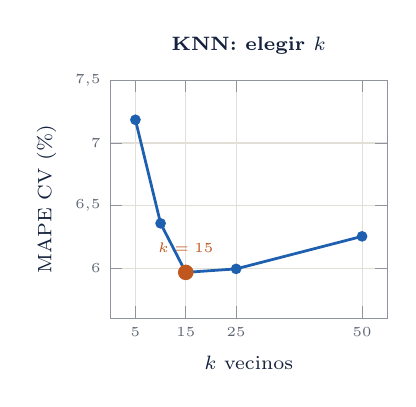
\begin{tikzpicture}
\begin{axis}[base, width=5.1cm, height=4.6cm, xmin=0, xmax=55, ymin=5.6, ymax=7.5,
  xtick={5,15,25,50}, xlabel={$k$ vecinos}, ylabel={MAPE CV (\%)}, title={KNN: elegir $k$}, grid=major,
  yticklabel style={/pgf/number format/fixed,/pgf/number format/precision=1}]
  \addplot[azul, line width=1pt, mark=*, mark size=1.4pt] coordinates {(5,7.186) (10,6.358) (15,5.966) (25,5.994) (50,6.254)};
  \addplot[only marks, mark=*, mark size=2.6pt, naranja] coordinates {(15,5.966)};
  \node[font=\tiny, text=naranja, anchor=south] at (axis cs:15,6.05) {$k = 15$};
\end{axis}
\end{tikzpicture}
\end{columns}
\vspace{0.1cm}
\centering\nota{Validación cruzada de 5 pliegues sobre el entrenamiento, con el MAPE como criterio.}
\end{frame}

% =====================================================================
% 11. Comparación con variabilidad
% =====================================================================
\begin{frame}{La regresión lineal múltiple gana}{Comparación de modelos}
\begin{columns}[c,onlytextwidth]
\column{0.58\textwidth}
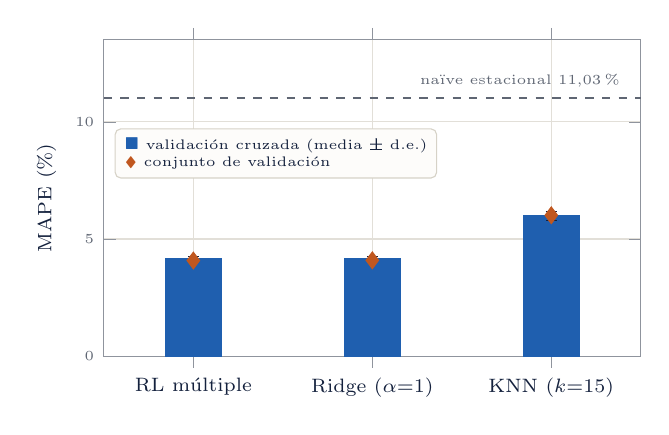
\begin{tikzpicture}
\begin{axis}[base, ybar, width=8.4cm, height=5.6cm, bar width=20pt, ymin=0, ymax=13.5,
  symbolic x coords={RL,Ridge,KNN}, xtick={RL,Ridge,KNN}, xticklabels={{RL múltiple},{Ridge ($\alpha$=1)},{KNN ($k$=15)}},
  x tick label style={font=\scriptsize, color=navy}, ylabel={MAPE (\%)}, enlarge x limits=0.25, grid=major]
  \addplot[fill=azul, draw=azul, error bars/.cd, y dir=both, y explicit, error bar style={navy, line width=0.8pt}]
    coordinates {(RL,4.17) +- (0,0.10) (Ridge,4.17) +- (0,0.10) (KNN,5.98) +- (0,0.18)};
  \addplot[only marks, mark=diamond*, mark size=3pt, naranja] coordinates {(RL,4.08) (Ridge,4.09) (KNN,6.01)};
  \draw[gris, dashed, line width=0.8pt] (rel axis cs:0,0.817) -- (rel axis cs:1,0.817) node[pos=0.98, above, font=\tiny, text=gris, anchor=south east] {naïve estacional 11,03\,\%};
  \node[font=\tiny, text=navy, anchor=north west, align=left, fill=tarjeta, draw=linea, rounded corners=2pt] at (rel axis cs:0.02,0.72)
    {{\color{azul}$\blacksquare$} validación cruzada (media ± d.e.)\\ {\color{naranja}$\blacklozenge$} conjunto de validación};
\end{axis}
\end{tikzpicture}
\column{0.39\textwidth}
\small
\begin{itemize}\setlength{\itemsep}{5pt}
  \item {\bfseries RL múltiple: 4,08\,\%} en validación, R$^2$ = 0,883.
  \item Ridge empata: la diferencia es menor que la variación entre pliegues (±0,10).
  \item KNN es peor en los 5 pliegues: 5,98\,\%.
  \item Los tres bajan con claridad del piso de 11,03\,\%.
\end{itemize}
\end{columns}
\end{frame}

% =====================================================================
% 12. Por qué MAPE
% =====================================================================
\begin{frame}{Por qué medimos con MAPE}{Métrica justificada por el costo}
\begin{columns}[T,onlytextwidth]
\column{0.48\textwidth}
\centering
{\color{navy}$\displaystyle \text{MAPE} = \frac{100}{n}\sum_{i=1}^{n}\frac{|\,\text{real}_i - \text{pronóstico}_i\,|}{\text{real}_i}$}
\vspace{0.25cm}

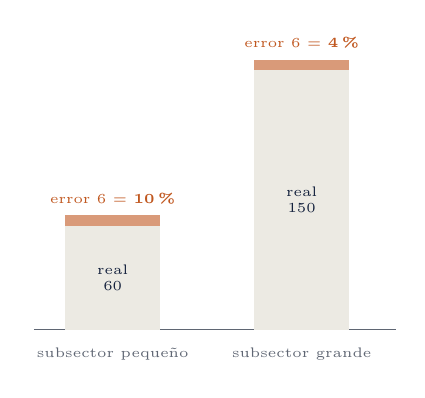
\begin{tikzpicture}[x=1cm,y=0.022cm]
  \draw[gris] (0,0) -- (4.6,0);
  \fill[grisc] (0.4,0) rectangle (1.6,60); \fill[naranja!60] (0.4,60) rectangle (1.6,66);
  \fill[grisc] (2.8,0) rectangle (4.0,150); \fill[naranja!60] (2.8,150) rectangle (4.0,156);
  \node[font=\tiny, text=navy, align=center] at (1.0,30) {real\\ 60};
  \node[font=\tiny, text=navy, align=center] at (3.4,75) {real\\ 150};
  \node[font=\tiny, text=naranja, anchor=south] at (1.0,67) {error 6 = \bfseries 10\,\%};
  \node[font=\tiny, text=naranja, anchor=south] at (3.4,157) {error 6 = \bfseries 4\,\%};
  \node[font=\tiny, text=gris] at (1.0,-14) {subsector pequeño};
  \node[font=\tiny, text=gris] at (3.4,-14) {subsector grande};
\end{tikzpicture}
\column{0.49\textwidth}
\small
\begin{itemize}\setlength{\itemsep}{4pt}
  \item El costo del error de inventario crece con el volumen de ventas: el mismo error pesa más en un subsector pequeño.
  \item Pronosticar de más deja inventario quieto; pronosticar de menos deja la tienda sin producto.
  \item {\bfseries Cuidado:} el MAPE castiga más el sobrepronóstico, que no tiene tope, que el subpronóstico, que llega como máximo al 100\,\%.
  \item Por eso lo acompañamos con MAE, RMSE y R$^2$.
\end{itemize}
\end{columns}
\end{frame}

% =====================================================================
% 13. Lectura del mejor modelo: errores
% =====================================================================
\begin{frame}{Los errores del mejor modelo no tienen sesgo}{Lectura del mejor modelo}
\begin{columns}[T,onlytextwidth]
\column{0.5\textwidth}
\begin{tikzpicture}
\begin{axis}[base, width=7cm, height=5.2cm, xmin=50, xmax=160, ymin=50, ymax=160,
  xlabel={Ventas reales (millones USD)}, ylabel={Pronóstico}, title={Pronóstico frente a real (validación, 1.080 filas)}, grid=major]
  \addplot[only marks, mark=*, mark size=0.55pt, azul, opacity=0.45] table[x=real,y=pred,col sep=comma] {datos/val_pred.csv};
  \addplot[naranja, dashed, line width=1pt, domain=50:160] {x};
\end{axis}
\end{tikzpicture}
\column{0.48\textwidth}
\begin{tikzpicture}
\begin{axis}[base, ybar interval, x tick label as interval=false, width=6.8cm, height=5.2cm, xmin=-18, xmax=20, ymin=0, ymax=200,
  xtick={-15,-10,-5,0,5,10,15}, xlabel={Residuo = real $-$ pronóstico}, ylabel={Filas}, title={Distribución de los errores}, grid=major]
  \addplot[fill=azul!55, draw=white] table[x expr=\thisrow{centro}-1, y=n, col sep=comma] {datos/hist_res.csv};
  \draw[naranja, line width=1pt] (axis cs:0,0) -- (axis cs:0,200);
\end{axis}
\end{tikzpicture}
\end{columns}
\vspace{0.05cm}
\centering\scriptsize
\dato{R$^2$ = 0,883}{} \quad·\quad \dato{MAE = 4,2}{millones} \quad·\quad \dato{error medio = $-0{,}06$}{} \quad·\quad \dato{48\,\%}{bajo lo real}
\end{frame}

% =====================================================================
% 14. Lectura: variables
% =====================================================================
\begin{frame}{Qué variables usa el modelo}{Interpretación preliminar}
\begin{columns}[T,onlytextwidth]
\column{0.56\textwidth}
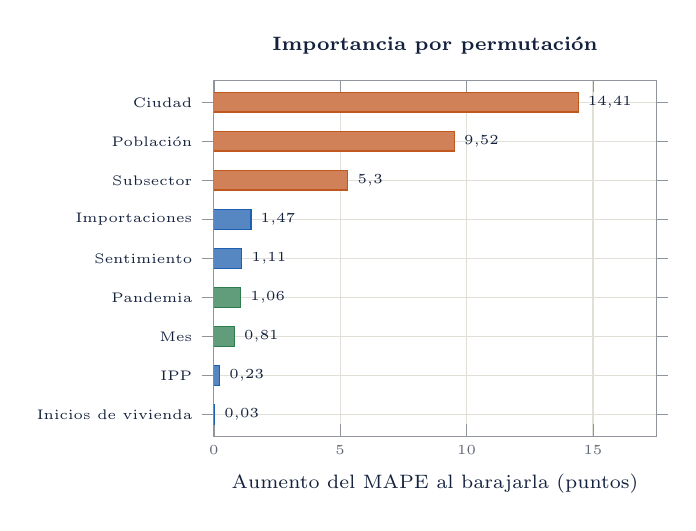
\begin{tikzpicture}
\begin{axis}[base, xbar, bar shift=0pt, width=7.2cm, height=6.1cm, bar width=7pt, xmin=0, xmax=17.5,
  symbolic y coords={inicios,ipp,mes,pandemia,sentimiento,importaciones,subsector,poblacion,ciudad},
  ytick={inicios,ipp,mes,pandemia,sentimiento,importaciones,subsector,poblacion,ciudad},
  yticklabels={Inicios de vivienda, IPP, Mes, Pandemia, Sentimiento, Importaciones, Subsector, Población, Ciudad},
  y tick label style={font=\tiny, color=navy}, xlabel={Aumento del MAPE al barajarla (puntos)},
  title={Importancia por permutación},
  nodes near coords, nodes near coords style={font=\tiny, color=navy, /pgf/number format/fixed, /pgf/number format/precision=2},
  nodes near coords align={horizontal}, grid=major, enlarge y limits=0.07]
  \addplot[fill=naranja!75, draw=naranja] coordinates {(14.41,ciudad) (9.52,poblacion) (5.30,subsector)};
  \addplot[fill=azul!75, draw=azul] coordinates {(1.47,importaciones) (1.11,sentimiento) (0.23,ipp) (0.03,inicios)};
  \addplot[fill=verde!75, draw=verde] coordinates {(1.06,pandemia) (0.81,mes)};
\end{axis}
\end{tikzpicture}
\column{0.41\textwidth}
\scriptsize
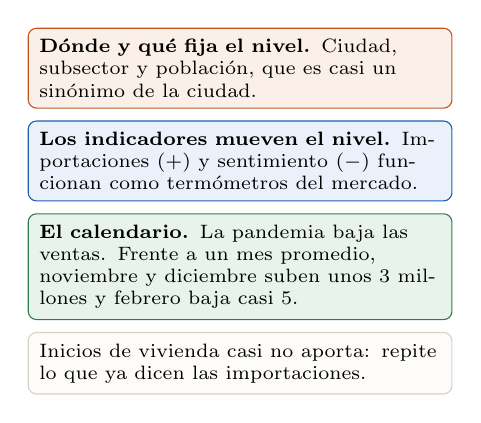
\begin{tikzpicture}
  \node[cajana, text width=5.1cm, align=left] (a) {{\bfseries Dónde y qué fija el nivel.} Ciudad, subsector y población, que es casi un sinónimo de la ciudad.};
  \node[cajaaz, text width=5.1cm, align=left, below=0.15cm of a] (b) {{\bfseries Los indicadores mueven el nivel.} Importaciones (+) y sentimiento ($-$) funcionan como termómetros del mercado.};
  \node[cajave, text width=5.1cm, align=left, below=0.15cm of b] (c) {{\bfseries El calendario.} La pandemia baja las ventas. Frente a un mes promedio, noviembre y diciembre suben unos 3 millones y febrero baja casi 5.};
  \node[caja, text width=5.1cm, align=left, below=0.15cm of c] (d) {Inicios de vivienda casi no aporta: repite lo que ya dicen las importaciones.};
\end{tikzpicture}
\end{columns}
\end{frame}

% =====================================================================
% 15. Robustez y limitaciones
% =====================================================================
\begin{frame}{¿Aguanta si pronosticamos un año nuevo?}{Prueba de robustez y limitaciones}
\begin{columns}[T,onlytextwidth]
\column{0.53\textwidth}
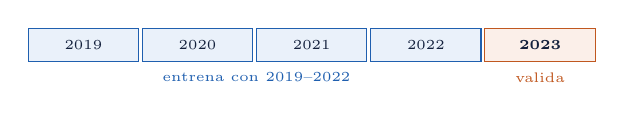
\begin{tikzpicture}[x=1cm,y=1cm]
  \foreach \a/\x in {2019/0,2020/1.45,2021/2.9,2022/4.35} \draw[fill=azulc, draw=azul] (\x,0) rectangle ++(1.4,0.42) node[midway,font=\tiny,text=navy] {\a};
  \draw[fill=naranjac, draw=naranja] (5.8,0) rectangle ++(1.4,0.42) node[midway,font=\tiny\bfseries,text=navy] {2023};
  \node[font=\tiny, text=azul, anchor=north] at (2.9,-0.02) {entrena con 2019–2022};
  \node[font=\tiny, text=naranja, anchor=north] at (6.5,-0.02) {valida};
\end{tikzpicture}

\vspace{0.1cm}
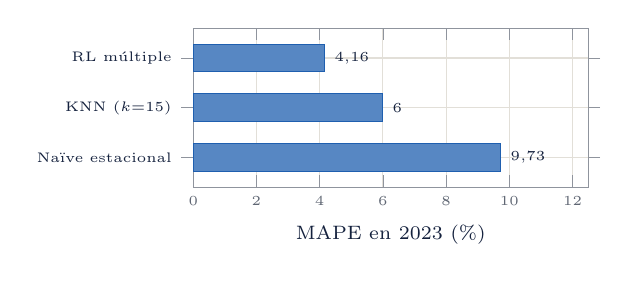
\begin{tikzpicture}
\begin{axis}[base, xbar, width=6.6cm, height=3.6cm, bar width=10pt, xmin=0, xmax=12.5,
  symbolic y coords={base,knn,mlr}, ytick={base,knn,mlr}, yticklabels={{Naïve estacional},{KNN ($k$=15)},{RL múltiple}},
  y tick label style={font=\tiny, color=navy}, xlabel={MAPE en 2023 (\%)}, enlarge y limits=0.3,
  nodes near coords, nodes near coords style={font=\tiny\bfseries, color=navy, /pgf/number format/fixed, /pgf/number format/precision=2},
  nodes near coords align={horizontal}, grid=major]
  \addplot[fill=azul!75, draw=azul] coordinates {(4.16,mlr) (6.00,knn) (9.73,base)};
\end{axis}
\end{tikzpicture}
\column{0.44\textwidth}
\scriptsize
{\color{naranja}\bfseries LIMITACIONES}
\begin{itemize}\setlength{\itemsep}{3pt}
  \item Los datos son simulados: los resultados dependen de los supuestos.
  \item La partición aleatoria mezcla meses; por eso hicimos esta prueba con un año completo nuevo.
  \item Las variables macro están muy correlacionadas entre sí.
\end{itemize}
\vspace{0.1cm}
{\color{naranja}\bfseries LO QUE SIGUE}
\begin{itemize}\setlength{\itemsep}{3pt}
  \item Abrir una sola vez el conjunto de prueba.
  \item Desplegar el modelo en Streamlit.
\end{itemize}
\end{columns}
\end{frame}

% =====================================================================
% 16. Conclusiones
% =====================================================================
\begin{frame}[plain]
\begin{tikzpicture}[remember picture,overlay]
  \fill[navy] (current page.south west) rectangle (current page.north east);
  \node[anchor=north west, text width=14cm, align=left] at ($(current page.north west)+(0.9,-0.75)$) {%
    {\color{azul!45}\fontsize{7.5}{9}\selectfont\bfseries CONCLUSIONES}\\[0.25cm]
    {\color{white}\fontsize{15}{18}\selectfont\bfseries Lo que dejamos listo en la Fase 2}};
  \node[anchor=north west, align=left, text=white, font=\small] at ($(current page.north west)+(0.9,-2.2)$) {%
    \renewcommand{\arraystretch}{1.25}%
    \begin{tabular}{@{}>{\color{azul!45}\bfseries}l@{\hspace{0.3cm}}p{13cm}@{}}
      1 & Una simulación fundamentada de 5.400 filas que reproduce la tendencia, la estacionalidad, la pandemia y las correlaciones del artículo.\\[5pt]
      2 & Un flujo sin fuga: Pipeline dentro de la validación cruzada y la prueba sellada.\\[5pt]
      3 & La regresión lineal múltiple gana: MAPE de 4,08\,\% frente a 11,03\,\% de la línea base. Como en el artículo, el modelo lineal es la mejor opción.\\[5pt]
      4 & El resultado se sostiene al pronosticar 2023 completo: MAPE de 4,16\,\%.
    \end{tabular}};
  \node[anchor=south west, text width=14cm, align=left] at ($(current page.south west)+(0.9,0.6)$) {%
    {\color{white}\fontsize{13}{15}\selectfont\bfseries Gracias}\\[0.1cm]
    {\color{white!65!azul}\fontsize{7}{9}\selectfont \integrantes\quad·\quad \repositorio}\\[0.08cm]
    {\color{white!55!azul}\fontsize{6}{8}\selectfont Usamos inteligencia artificial generativa como apoyo; el equipo revisó cada cifra y puede sustentar cada decisión.}};
\end{tikzpicture}
\end{frame}

\end{document}
